\documentclass{beamer}

\usepackage{siunitx}
\usepackage{bm}
\usetheme{default}
\usecolortheme{CVUTFIT}
\beamertemplatenavigationsymbolsempty
\setbeamertemplate{footline}[frame number]

\title{Laserová spektroskopie magneticky uspořádaných materiálů}
\author{Vladislav Wohlrath}
\institute{Matematicko-fyzikální fakulta UK\\ \vspace{0.2cm} Katedra chemické fyziky a optiky (KChFO) \\ \vspace{0.2cm} Vedoucí: prof. RNDr. Petr Němec, Ph.D. \\ \vspace{0.3cm} Konzultace teorie: doc. RNDr. Tomáš Ostatnický, Ph.D.}
\date{16. června 2022}


\begin{document}
\frame[plain]{\titlepage}

\begin{frame}{Motivace a kontext}
\begin{itemize}
    \item Materiálový výzkum pro spintroniku
        \begin{itemize}
            \item Pro spintroniku důležité magnetické materiály
        \end{itemize}
        \pause
        \item Probíhající experiment v laboratoři optospintroniky (LOS)
            \begin{itemize}
                \item Metoda studia magneticky uspořádaných materiálů pomocí kvadratických magneto-optických jevů ($\propto \bm{M}^2$)
        \begin{itemize}
            \item Širší třída materiálů než lineární ($\propto \bm{M}$) -- antiferomagnety
        \end{itemize}
        \pause
                \item Předchozí práce
                    \begin{itemize}
                        \item Kimák, bakalářská práce 2017
                        \item Wohlrath, bakalářská práce 2018
                        \item Kubaščík, bakalářská práce 2019
                        \item Kimák, diplomová práce 2019
                    \end{itemize}
                    \pause
                \item Nekonzistentní výsledky
            \end{itemize}
        \item \textbf{Cíl práce:} identifikovat problémy, případně je odstranit
    \end{itemize}
\end{frame}

\begin{frame}{Popis experimentu}
    \begin{itemize}
        \item 2-D elektromagnet, v rovině vzorku (transversální pole)
            \begin{itemize}
                \item Změna směru magnetického pole o konstantní velikosti
            \end{itemize}
            \visible<2->{\item Detekce stočení polarizace (schéma optického můstku)}
        \visible<3>{\item (Téměř) kolmý dopad a transversální magnetizace
        \begin{itemize}
            \item Vymizení lineárních jevů
    \end{itemize}}
    \end{itemize}
    \vspace{0.3cm}
    \hspace{1cm}
    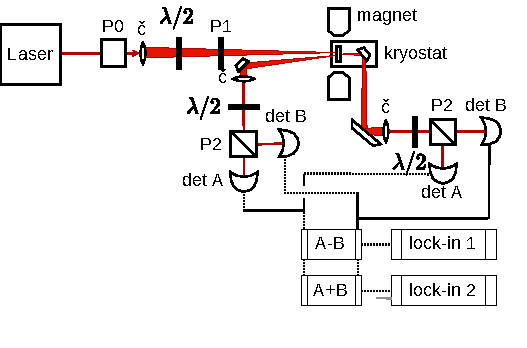
\includegraphics{img/schema-hlavni.drawio.pdf}
\end{frame}

\begin{frame}{Popis experimentu}
    \begin{columns}
        \begin{column}{0.55\textwidth}
            
    \begin{enumerate}
        \item Nastavená vlnová délka $\lambda$
        \item<2-> Rotující vnější pole $\varphi_{H} \in (\SI{0}{\degree},\SI{360}{\degree})$
        \item<3-> Měřeno stočení polarizace $\Delta\beta$
        \item<4-> Opakováno pro různé vstupní polarizace $\beta$
        \visible<5->{\item Očekávaná závislost $\Delta\beta = P \sin 2 (\varphi_M - \beta)$
            \begin{itemize}
                \item Určení $P(\lambda)$ a $\varphi_M(\varphi_H)$
                \item<6-> \textbf{Problém}: nekonzistence napříč $\lambda$
        \end{itemize}}
    \end{enumerate}
        \end{column}
        \begin{column}{0.45\textwidth}
            \visible<4->{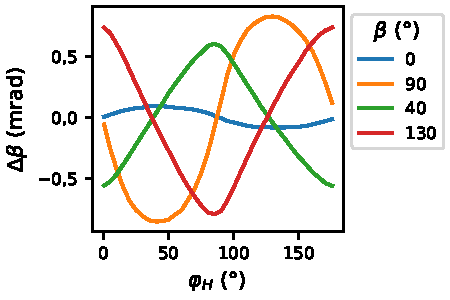
\includegraphics[width=\textwidth]{img/def1.pdf}}
        \visible<5->{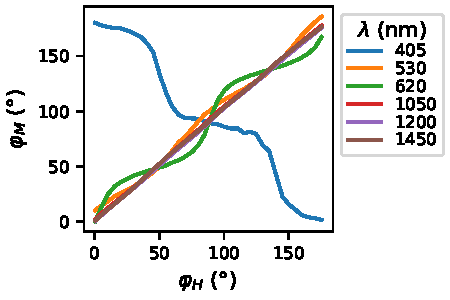
\includegraphics[width=\textwidth]{img/def2.pdf}}
        \end{column}
\end{columns}
\end{frame}



\begin{frame}{Řešení}
    \begin{itemize}
        \item Objeveno několik problémů
            \begin{enumerate}
                \item Optika
                    \only<1-4>{\begin{itemize}
                        \item $\lambda/2$ vlnové destičky nemají fázové zpoždění přesně $\pi/2$

                        \item Zrcadla zanáší fázové zpoždění mezi s- a p- (pokrytí)
                        \item<2-> Oba problémy způsobují, že měřený signál neodpovídá čisté rotaci polarizace ($\Delta\beta$), ale v podstatě náhodnému mixu rotace a elipticity (tj. jinou projekci komplexní Kerrovy rotace)
                        \item<3-> Nutná buď kompenzace nebo charakterizace
                        \item<4-> Navrženo a vyzkoušeno několik metod, vybrána ta nejjednodušší
                \end{itemize}
            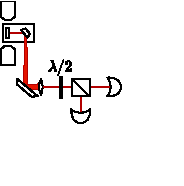
\includegraphics[width=1.5in]{img/mustek.drawio.pdf}}
        \item<5-> Magneto-optika
            \only<5-7>{\begin{itemize}
                        \item<5-> Dříve používaný vzorec $\Delta\beta = P \sin 2 (\varphi_M - \beta)$ neplatí pro krystaly
                        \item<6-> Důkladné přezkoumání relevantní fyziky $\Rightarrow$ vzorec platný pro kubický vzorek s normálou [001] ($\gamma = $ úhel in-plane rotace) $\Delta\beta = P_+ \sin 2 (\varphi_M - \beta) +  P_- \sin 2 (-\varphi_M - \beta+2\gamma)$
                        \item<7-> Po mnoha stránkách vylepšena metodika zpracování dat
                \end{itemize}}
            \item<8-> Další problémy
            \only<8-9>{\begin{itemize}
                \item<8-> Nepřesnosti v magnetickém poli
                \item<9-> Dodatečné MO jevy pocházející od okénka kryostatu -- odstranění na základě rozdílné symetrie
        \end{itemize}}
            \end{enumerate}
        \item<10-> Všechny problémy vyřešeny
        \visible<11->{
        \item Ověření funkčnosti metody s feromagnetickými vzorky
            \begin{itemize}
                \item Transmisní geometrie: CoFe -- \SI{295}{K}, \SI{15}{K}
                \item Reflexní geometrie: FeRh -- \SI{420}{K}
            \end{itemize}
        }
    \end{itemize}
\end{frame}



\begin{frame}{Výsledky -- CoFe}
    \begin{itemize}
        \item Magnetická anizotropie změřená různými vlnovými délkami se velmi přesně shoduje $\Rightarrow$ důkaz funkčnosti
            \pause
        \item Shoduje se i s výsledky poskytnutými výrobcem vzorku (torque-metrie)
            \pause
        \item Funkcionál magnetické volné energie
            \begin{itemize}
                \item Určení snadných/těžkých os magnetizace (minima $F$)
            \end{itemize}
        \item<4> Slabá závislost na teplotě
    \end{itemize}
    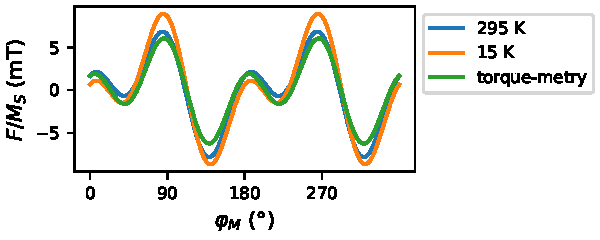
\includegraphics{img/cofe-funkcional.pdf}    
\end{frame}


\begin{frame}{Výsledky -- CoFe}
    \begin{itemize}
        \item Spektrum MO koeficientů (izotropní $P_+$ a anizotropní $P_-$)
        \item<2-> Slabá závislost na teplotě
        \item<3-> Změna znaménka obou koeficientů
        \item<4-> ``Maximální anizotropie'': $P_+=0$, $P_+=P_-$, $P_+=-P_-$
            \begin{itemize}
                \item<3-> Dosaženo ve viditelné oblasti
            \end{itemize}
   \end{itemize} 
   \vspace{0.1cm}
   \hspace{0.1cm}\begin{center}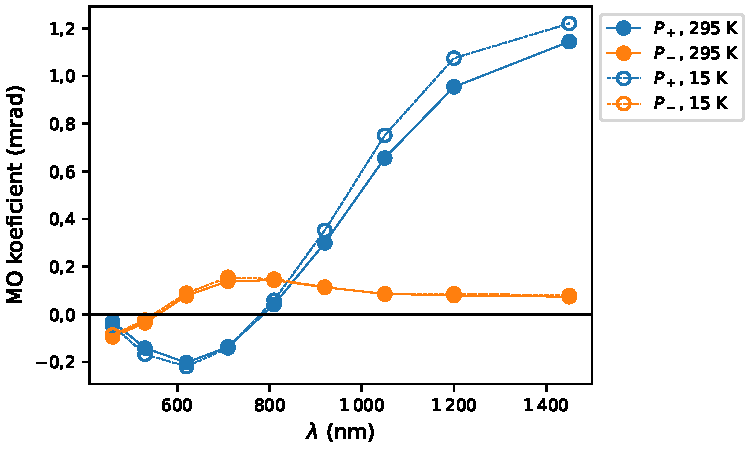
\includegraphics[width=0.8\textwidth]{img/cofe-pmld.pdf}\end{center}
\end{frame}

\begin{frame}{Výsledky -- FeRh}
    \begin{itemize}
        \item Spektrum MO koeficientů
            \begin{itemize}
                \item<2-> Vysoká anizotropie ($P_+=0$, $P_+=P_-$, $P_+=-P_-$)
                \item<3-> Velmi silná spektrální závislost
            \end{itemize}
    \end{itemize}
    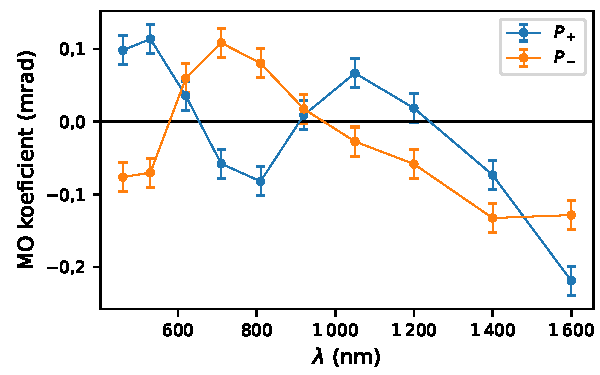
\includegraphics{img/ferh-pmld.pdf}
\end{frame}

\begin{frame}{Výsledky}
    \begin{itemize}
        \item Všechny problémy opraveny a metoda je konzistentní
            \pause
        \item Určení magnetické anizotropie ($\bm{M}(\bm{H}_{\textrm{ext}})$) pouze z kvadratických jevů
            \begin{itemize}
                \item V literatuře nepublikován
            \end{itemize}
            \pause
        \item Není nutné otáčet vzorek $\Rightarrow$ možnost použití kryostatu
            \begin{itemize}
                \item V literatuře nepublikován
            \end{itemize}
            \pause
        \item Otevřené dveře pro použití metody k výzkumu antiferomagnetů
            \begin{itemize}
                \item Již probíhá (Zeynab Sadeghi)
            \end{itemize}
            \pause
        \item Změřená silná anizotropie kvadratického MO jevu se silnou spektrální závislostí
            \begin{itemize}
                \item \textbf{Důsledky pro ostatní metody}, které ho využívají (a často zanedbávají anizotropii)
                    \begin{itemize}
                        \item Pump and probe metody, studium hysterezních smyček, \ldots
                    \end{itemize}
            \end{itemize}
    \end{itemize}
\end{frame}
% Vedlejší přínosy
\input{vedlejsi.tex}


\begin{frame}{Shrnutí}
    \begin{itemize}
        \item Konečné opravení dlouhodobě problematické metody studia kvadratických MO jevů ve feromagnetech
            \begin{itemize}
                \item Problém se zrcadly měnícími polarizaci
                \item Správné pochopení kvadratických MO jevů $\Rightarrow$ opravený způsob zpracování dat
            \end{itemize}
            \pause
        \item Demonstrace a první úspěšné použití metody
            \begin{itemize}
                \item Transmisní geometrie: CoFe
                \item Reflexní geometrie: FeRh
                \item První experimenty svého druhu s kryostatem
            \end{itemize}
            \pause
        \item Změřena silná anizotropie kvadratického jevu
            \begin{itemize}
                \item Důsledky pro ostatní metody využívající kvadratické MO jevy (pump-probe, studium hysterezních smyček, \ldots)
            \end{itemize}
            \pause
        \item Využití pro studium antiferomagnetů
    \end{itemize}
\end{frame}

% Otázky oponenta
\begin{frame}{Otázky oponenta}
    \begin{block}{Otázka 1a)}
        V práci zavádíte zobrazení intenzit Stokesova vektoru plně polarizovaného světla na
        Poincarého sféře (obr. 1.3).
        V práci dále řešíte odezvu optického můstku sestávajícího z fázové destičky, polarizačního děliče a dvojice detektorů, přičemž můstek je nastaven tak, aby rozdíl signálů z obou detektorů byl nula (kapitola 4.2).
        Množina polarizací, které poskutují nulový signál z ideálního optického můstku je pak znázorněna poledníkem mezi pólem kruhových polarizací a polarizací 0-\SI{90}{\degree} (obr. 4.3).
        Můžete prosím graficky ukázat, jak se tato množina nulové odezvy změní, když můstek nebude sestaven z opticky ideálních elementů?
        Např. když zpoždění fázové destičky nebude přesně $\pi/2$, či fázová destička bude mít různou propustnost pro obě vlastní polarizace?
    \end{block}
\end{frame}

\begin{frame}{Otázky oponenta}
    \begin{block}{Otázka 1a)}
        [Množiny nulové odezvy pro neideální fázovou destičku?]
    \end{block}
    \begin{exampleblock}{Odpověď 1a)}
        \begin{columns}
            \begin{column}{0.5\textwidth}
                \begin{itemize}
                    \item Nepřesné fázové zpoždění
                    \item Vyklopení do $s_3$ 
                \end{itemize} 
                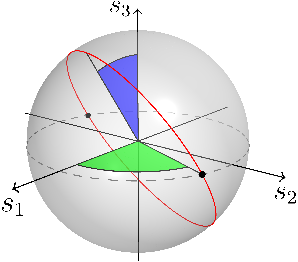
\includegraphics[width=4cm]{img/kovek-4.pdf}
            \end{column}
            \begin{column}{0.5\textwidth}
                \begin{itemize}
                    \item Rozdílná propustnost
                    \item Posunutí v rovině $s_1s_2$
                \end{itemize} 
                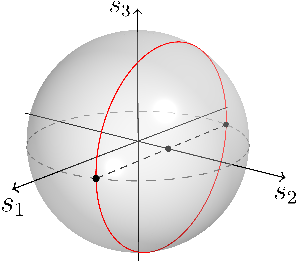
\includegraphics[width=4cm]{img/kovek-6.pdf}
            \end{column}
        \end{columns}
    \end{exampleblock}
\end{frame}

\begin{frame}{Otázky oponenta}
    \begin{block}{Otázka 1b)}
        Jak se v této vizualizaci projeví, když např. k s-polarizovanému světlu na vstupu (($\beta=0$) a optický můstek je vyvážen) je přičtena např. Kerrova rotace a optický můstek tedy přestane být vyvážen?
    \end{block}
    \begin{exampleblock}{Odpověď 1b)}
        \begin{itemize}
            \item Stokesův kovektor zůstane nezměněný -- stav detekční aparatury (můstku) se nezměnil
            \item Změní se Stokesův vektor -- vstupní světlo se změnilo právě o Kerrovu rotaci
            \item Detekovaný signál je dán ``vzdáleností'' bodu od kružnice
        \end{itemize}
    \end{exampleblock}
\end{frame}

\begin{frame}{Otázky oponenta}
    \begin{block}{Otázka 1b)}
        [Jak se projeví Kerrova rotace (rozvážení můstku)?]
    \end{block}
    
    \begin{exampleblock}{Odpověď 1b)}
        \begin{columns}
            \begin{column}{0.5\textwidth}
                \begin{itemize}
                    \item Nepřesné fázové zpoždění
                    \item Vyklopení do $s_3$ 
                    \item V signálu se projeví elipticita
                \end{itemize} 
                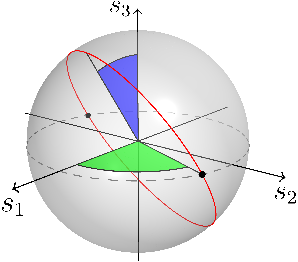
\includegraphics[width=4cm]{img/kovek-4.pdf}
            \end{column}
            \begin{column}{0.5\textwidth}
                \begin{itemize}
                    \item Rozdílná propustnost
                    \item Posunutí v rovině $s_1s_2$
                    \item Snížení faktoru stočení
                \end{itemize} 
                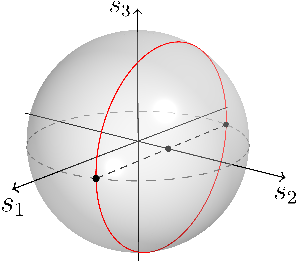
\includegraphics[width=4cm]{img/kovek-6.pdf}
            \end{column}
        \end{columns}
    \end{exampleblock}
\end{frame}

\begin{frame}{Otázky oponenta}
    \begin{block}{Otázka 2)}
        Při zpracování magnetooptických spekter CoFe je oddělena magnetooptická odezva (např. určení spekter amplitudy a anizotropie magnetooptického jevu) a magnetická odezva (určení snadných os a magnetické anizotropie), obr. 5.2.
        V tomto zpracování je magnetická anisotropie určena pro různé vlnové délky světla, což není fyzikálně přesné, ale indikuje správnost oddělení obou jevů.
        Bylo by možné modifikovat formalismus zpracování dat, aby bylo zcela odděleno magnetické chování vzorku (tj. stejné chování pro všechny vlnové délky světla) a magneto-optická spektrální odpověď vzorku?
    \end{block}
\end{frame}
\begin{frame}{Otázky oponenta}
    \begin{block}{Otázka 2)}
        [Oddělené zpracování magnetické a magneto-optické odezvy?]
    \end{block}
    
    \begin{exampleblock}{Odpověď 2)}
        \begin{itemize}
        \item Analýza $\equiv$ globální minimalizace chybové funkce $\mathcal{L} = \sum \left( U_{\textrm{experiment}} - U_{\textrm{model}} \right)^2$, kde $U_{\textrm{model}}(\textrm{M},\,\textrm{MO})$
        \item Je možné zpracovávat všechny vlnové délky zároveň, pak $U_{\textrm{model}}(\textrm{M},\,\textrm{MO}(\lambda_1),\,\textrm{MO}(\lambda_2),\,\ldots)$
                \begin{itemize}
                    \item Různé $\lambda$ mají různou hladinou šumu, je nutné to zohlednit přidáním vah do chybové funkce $\mathcal{L}=\sum_\lambda w^2(\lambda) \left(U_{\textrm{experiment}} - U_{\textrm{model}}\right)^2$
                    \item Pokud jsou výsledky podobné (v jejich rozsahu je model přibližně lineární) je to ekvivalentní váženému průměru výsledků jednotlivých $\lambda$
                    \item Vyzkoušeno, ale kvůli předchozímu bodu nepoužíváno
                \end{itemize}
        \end{itemize}
    \end{exampleblock}
    
\end{frame}




\end{document}
